\documentclass[ipc]{suribt}
%\documentclass[oneside]{suribt}% 本文が * ページ以下のときに (掲示に注意)
\title{電力制約下における蓄電池を用いた高性能計算システムの性能向上}
%\titlewidth{}% タイトル幅 (指定するときは単位つきで)
\author{酒井 崇至}
\eauthor{Takayuki Sakai}% Copyright 表示で使われる
\studentid{03-120601}
\supervisor{中村 宏 教授}% 1 つ引数をとる (役職まで含めて書く)
%\supervisor{指導教員名 役職 \and 指導教員名 役職}% 複数教員の場合,\and でつなげる
\handin{2014}{2}% 提出月. 2 つ (年, 月) 引数をとる
%\keywords{キーワード1, キーワード2} % 概要の下に表示される

\usepackage{graphicx}
%\graphicspath{{./fig/}}
\usepackage{amsmath}

\begin{document}
\maketitle%%%%%%%%%%%%%%%%%%% タイトル %%%%

\frontmatter% ここから前文
\begin{abstract}%%%%%%%%%%%%% 概要 %%%%%%%%
近年、コンピュータの消費電力の増大が大きな問題となっている。そのためコンピュータの性能の指標として単なる実行速度だけではなく、消費電力あたりの実行速度が重要視されるようになってきている。特にスーパーコンピュータのような今日の高性能計算システムでは数メガワットもの電力を消費しており、物理的制約からこれ以上の電力供給力の向上は困難である。このような背景により、予め決められた消費電力の制約下での実行速度の最大化が、今後の高性能計算システムの性能向上の鍵となっている。

そこで、本論文では蓄電池を用いた高性能計算システムの電力制約下での性能向上手法を提案する。現在の高性能計算システムには、停電時にもシステムへの電力供給を続けられるようにUPS(無停電電源装置)が搭載されている。それを非停電時にも積極的に充放電を行い、アプリケーションの中の電力をかけても性能が上がりにくい部分から上がりやすい部分へ、電力を時間方向に融通することによって、電力制約下における性能を向上させることができる。本研究ではCPU-GPUハイブリッド構成の計算ノードを用いて、CPU上での並列アプリケーション及びGPU上での並列アプリケーションから2種類ずつのベンチマークを選び、本手法を用いた場合の性能評価実験を行った。その結果、本手法を上手く適用できるアプリケーションに関しては、本手法を用いない場合に比べてCPU上での並列アプリケーションでは平均4.5\%、GPU上での並列アプリケーションでは平均17.1\%の性能向上が実現できることを示し、その有用性を確認した。

\end{abstract}

\tableofcontents%%%%%%%%%%%%% 目次 %%%%%%%%

\mainmatter% ここから本文 %%% 本文 %%%%%%%%

\chapter{序論}

現代社会においてコンピュータの担う役割はかつてないほど大きくなっており、我々の生活に欠くことのできない存在となっている。より高性能なコンピュータを作るべく、これまで多くの研究者がコンピュータ技術の発展に貢献し、Mooreの法則\cite{mooreslaw}の示す通りチップの集積度が指数関数的に増すと共にコンピュータの性能も向上し続けている。

近年、コンピュータの性能向上の妨げとなっている要因の一つが消費電力の増大である。一般に、電力を多く消費するほど高速な演算を行いやすいという傾向があり、数年前までは性能向上と共に消費電力も増加し続けてきた。ところがスーパーコンピューターなどのHPC領域においては既に供給できる限界に近い電力を消費しており、物理的な電力供給能力によってコンピュータの性能が制限されてしまうことが懸念されている。そのため、与えられた電力制約の中でいかに処理能力を向上させるかが現在の大きな課題となっている。

この課題に対抗して電力対性能を向上させるため、プロセッサやメモリの動作速度を動的に制御する技術が開発され、現在の多くのコンピュータに搭載されている。この技術は性能のクリティカルパス上にないモジュールの動作速度を落とすことにより、性能低下を防ぎつつ消費電力を下げるというものであり、この技術の成熟による電力対性能の向上が期待されている。

また、現在のデータセンターやスーパーコンピュータなどの大規模高性能計算システムにおいては、BCM(事業継続マネジメント)の観点から、地震や火事などの災害による停電時にも継続してコンピュータを稼働させられるように自家発電設備や蓄電池が搭載されているケースが多くなってきた。ただ、現状ではそれらの設備はあくまで緊急時のための予備電源としてのみ見なされており、平常時には使用されていない。そのため、それらの新たな電力資源を有効活用して電力対性能を向上させることができると提案されている\cite{Govindan:2011:BLT:2024723.2000105}が、まだこの可能性が示唆されてから日が浅く、特にHPCの領域においてはまだ未開拓の領域が多く残されている。

そこで本論文では、蓄電池が搭載された高性能計算システムにおいて非停電時にも積極的に蓄電池の充放電を行うことによって、電力制約下での性能向上手法を提案する。HPC領域において蓄電池を用いた電力対性能向上手法はいまだ提案されておらず、本稿において初めての試みである。

本手法では、アリゾナ大学のTapasya Patki氏らの研究\cite{Patki:2013:EHO:2464996.2465009}の対象となっているような、厳しい電力制約のために全てのモジュールを最高動作速度で動作させることができないようなシステムを対象とする。まずアプリケーションのテスト実行時のプロファイルデータからアプリケーションの電力対性能グラフの時間推移を予測する。そして消費電力を減らしても性能が下がりにくい部分を見つけて充電し、逆に消費電力を増やすと大きく性能が上がる部分で放電することにより、電力制約下における性能向上を目指す。

以降、2章では本論文に関する技術や研究を紹介し、3章では解くべき問題の定義と、提案手法の核となる論理を説明する。4章では3章での手法の有用性を確認するための実験方法について述べる。5章で実験結果を示し、6章でその結果について考察した後、7章で結論と今後の課題を述べる。


%\section{背景}
%\label{sec:background}


%\section{目的}


%\section{本論文の構成}


\chapter{関連研究}
\label{chap:background}



\section{DVFS}
\label{sec:dvfs}


\section{UPSを含む電力供給システム}
\label{sec:ups}


\section{パワーキャッピング手法}
\label{sec:capping}


\chapter{蓄電池を用いた高速化手法}
\label{chap:proposal}

前章でデータセンタにおける電力コスト削減要請についての背景および関連研究を紹介した。実は電力削減はデータセンタだけに限らず、コンピュータアーキテクチャ全体の共通の課題である。その中でもHPC(High Perfomance Computing)領域においては消費される電力は物理的制約による供給可能電力に達しつつあり、近い将来スーパーコンピュータの性能は電力供給能力によって頭打ちになると予想されている。そのため電力対性能の高いシステムの構築が必要とされている。本章ではその実現手法のひとつとして、既存設備に含まれるバッテリーを用いた電力対性能の向上手法を提案する。


\section{フェーズ間の電力融通手法の提案}
\label{sec:curb}

スーパーコンピュータ上で走るアプリケーションは実行時間が長く、実行が進むにつれて処理の特性が大きく変化するものも多い。CPUによる演算中心の処理やデータの読み書きなどのI/Oが中心の処理、プロセス間の通信が中心の処理など、異なる処理は基本的に異なる特性を持っている。また同じ処理であっても演算の並列度などの他の多くの要因に処理の特性は影響される。一般に処理の特性が異なると、その処理にかける電力と処理を終えるまでの実行時間の関係を表した電力ー実行時間曲線は異なったものになる。異なる電力ー実行時間曲線において、かける電力を変化させたときの実行時間時間の変動の大きさは異なる(図\ref{fig:power_time_proposal})。

\begin{figure}[t]
 \begin{center}
  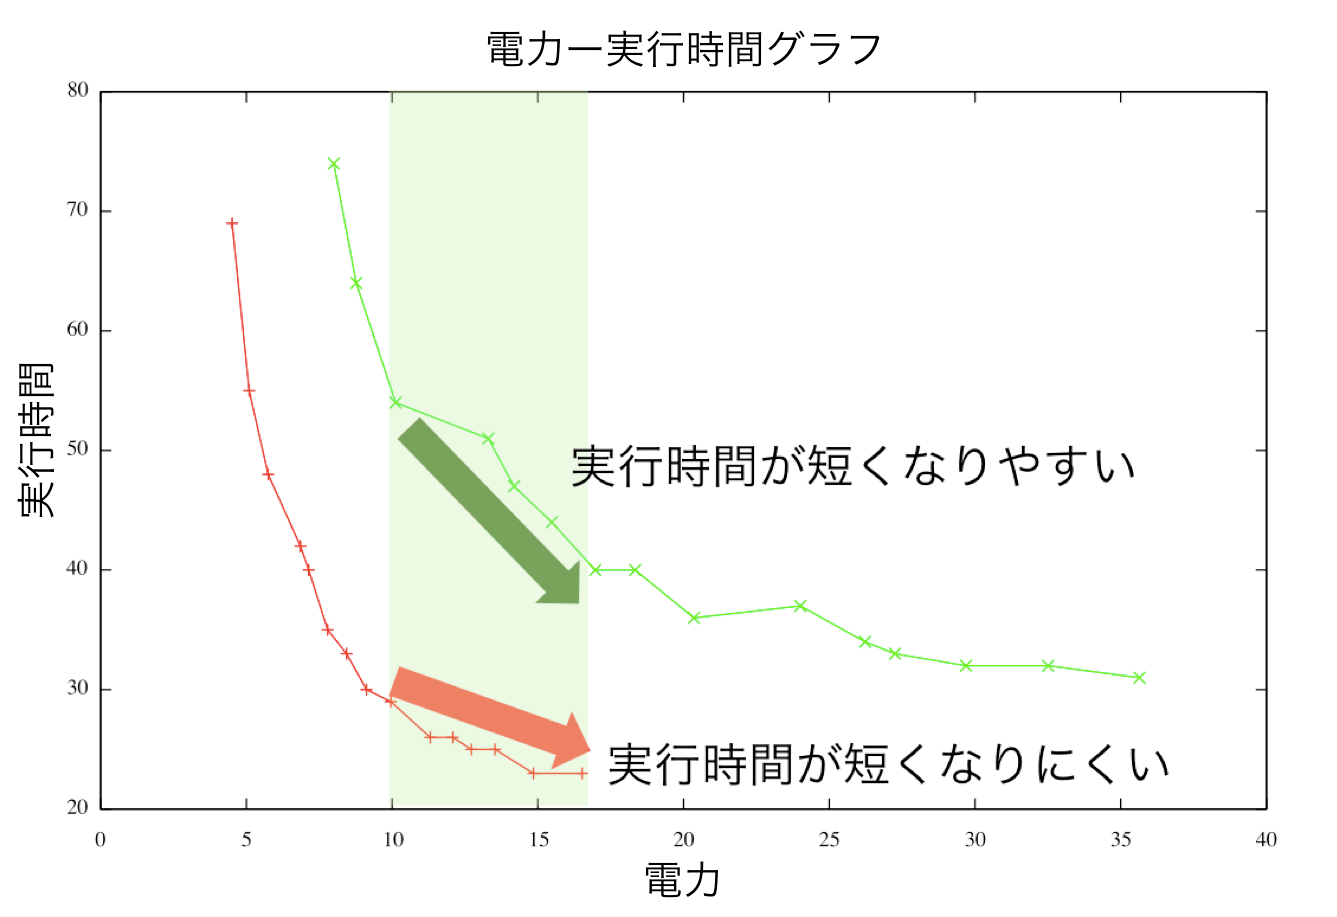
\includegraphics[width=110mm]{power_time_proposal.png}
 \end{center}
 \caption{電力ー実行時間曲線の違いによって、かける電力の増加による短縮される実行時間が異なる様子}
 \label{fig:power_time_proposal}
\end{figure}

本手法では処理の特性の違いによる電力ー実行時間曲線の違いに着目する。ひとつのアプリケーションを異なった処理の特性を持った時間的に連続する複数の区間に分割し、かける電力を減らしても実行時間があまり短くならない区間から、電力を多くかけると実行時間が大きく短くなる区間へ蓄電池を用いて時間方向へ電力を融通することにより実行時間を短縮する。

また、現在のプロセッサは離散的な有限の数の周波数でしか動作することはできない。そのため、電力制約によって最高周波数で動作できない場合であっても、使い切れていない電力というものが存在する。例えば、消費電力80Wおよび60Wの2種類の動作周波数をサポートしているプロセッサに対して70Wの電力制約をかけた場合、プロセッサは消費電力60Wの周波数でしか動作することができないので、10Wの電力を使い切れないことになる。蓄電池を用いればこの余った電力も時間方向に融通することで活用することができるので、その分実行時間の短縮に繋がると考えられる。

以上の実行区間ごとの電力ー実行時間曲線の違いを利用した性能向上と、動作周波数が離散的であることによる余剰電力を利用した性能向上が本論文における提案手法である。次節以降では、アプリケーションの区切り方および電力融通をどう行うかについての各論を述べる。


\section{フェーズの要件}
\label{sec:phase1}

節\ref{sec:curb}で述べたように、本手法では処理ごとの電力ー実行時間曲線の違いを利用して性能を向上させる。そのため、電力ー実行時間曲線の異なる区間をそれぞれ別のフェーズとして定義する。フェーズの区切り方が細かいほど電力融通の機会は増えることになるので、理想的なバッテリーを用いる場合には、アプリケーション内の電力ー実行時間曲線が異なる区間全てを別のフェーズとして区切る場合が理想的なフェーズの区切り方となる。

しかし、実際のバッテリーはあまり高頻度に充放電を行えない・充放電の速度に限界があるなど様々な物理的制約がある。また、フェーズの数が多くなるほど節\ref{sec:formularization}で述べる電力融通問題を解くことが困難になる。さらに、入力データが異なる場合には処理の順序が異なるので、どの時刻にどの処理が行われているかが分かりにくく、アプリケーション内の電力ー実行時間曲線が異なる部分を全て求めること自体も難しい問題である。そのため、現実の問題を扱う場合には電力ー実行時間曲線が異なる全ての部分ではなく、もっと粗い粒度でフェーズを区切ることになる。

\section{フェーズの求め方}
\label{sec:phase2}

HPC領域において、アプリケーションの性質や演算装置の特徴に応じてソースコードに手を加えることは珍しいことではない。ソースコードに手を加えるときに手間となるのはソースコードを書き直すことである。以下のコードはCPU並列化プラットフォームのOpenMPのコードであるが、このようにいくらかのコードを書き足す程度であればプログラマの大きな負担にはならない。

{\small
\begin{itembox}[c]{OpenMPのソースコード}
\begin{verbatim}
int main(int argc, char *argv[])
{
    int i;
#pragma omp parallel for       //性能向上のために追加される唯一の行
    for(i = 0; i <= 10000; i++)
    {
        // (並列処理させたいプログラム)
    }
}
\end{verbatim}
\end{itembox}}

本手法では、上の例のようにユーザプログラマにいくらかのコードを足してもらうことによりフェーズを区切る。具体的には以下のようになる。

{\small
\begin{itembox}[c]{本手法で想定するフェーズの指定方法}
\begin{verbatim}
int main(int argc, char *argv[])
{
#phase start A    //フェーズAの始まりを示す
    //フェーズAの処理
#phase end A      //フェーズAの終わりを示す
    //何らかの処理(ない場合もある)
#phase start B    //フェーズBの始まりを示す
    //フェーズBの処理
#phase end B      //フェーズBの終わりを示す
}
\end{verbatim}
\end{itembox}}

この区切りを示すコードは、時系列的に異なる処理の部分に配置さえされていれば、以下のように繰り返し文の中に入っていたり、他の関数にまたがっていたりしても構わない。

{\small
\begin{itembox}[c]{繰り返し文における例}
\begin{verbatim}
int main(int argc, char *argv[])
{
for(i = 0; i <= 10000; i++)
{
    #phase start A    //フェーズAの始まりを示す
        //フェーズAの処理
    #phase end A      //フェーズAの終わりを示す
    #phase start B    //フェーズBの始まりを示す
        //フェーズBの処理
    #phase end B      //フェーズBの終わりを示す
    }
}
\end{verbatim}
\end{itembox}}

{\small
\begin{itembox}[c]{関数にまたがっている場合の例}
\begin{verbatim}
functionA()
{
#phase start A    //フェーズAの始まりを示す
    //フェーズAの処理
#phase end A      //フェーズAの終わりを示す
}

functionB()
{
#phase start B    //フェーズBの始まりを示す
    //フェーズBの処理
#phase end B      //フェーズBの終わりを示す
}

int main(int argc, char *argv[])
{
    functionA();
    functionB();
}
\end{verbatim}
\end{itembox}}


\section{電力融通問題の定式化}
\label{sec:formularization}

節\ref{sec:phase2}の手法によってアプリケーションが$n$個のフェーズに区切られていて、それぞれのフェーズが1から$n$までの番号を一意に割り振られている状況を考える。フェーズ$i$(ただし$1\leq i\leq n$)における電力ー実行時間曲線を$T_i(p)$と定義する。$T_i(p)$はフェーズ$i$にかける電力$p$に対して、フェーズ$i$を終えるのにかかる実行時間を返す関数である。$T_i(p)$はフェーズ分割が行われていれば、それぞれのDVFSパターンについてテスト実行を行うことで得ることができる。この点については節\ref{sec:method}で詳しく述べる。

本論文での目的は、与えられた電力制約下においてアプリケーション全体の実行時間を最小化することである。そこで、与えられる電力制約を$p_{max}$とする。そして本手法ではフェーズごとに蓄電池を用いて電力を融通するため、フェーズ$i$において蓄電池から供給される電力を$\Delta p_i$とする。$\Delta p_i$はマイナスのときは蓄電池に充電することを意味する。

以上の変数を用いて最適化問題として定式化すると、以下のようになる。

\begin{eqnarray}
{\rm min } & \sum_{i=1}^n T_i(p_{max} + \Delta p_i) \label{asm:min} \\
{\rm s.t. } & \sum_{i=1}^n \Delta p_i T_i(p_{max} + \Delta p_i) \leq 0 \label{asm:s.t.}
\end{eqnarray}

式(\ref{asm:min})は実行時間の最小化を意味する。式(\ref{asm:s.t.})の左辺は、アプリーケション実行の全体を通して、蓄電池から供給されるエネルギを意味している。蓄電池はあくまで電力を時間方向に融通しているだけであり、エネルギを増やすことはできない。そのため、式(\ref{asm:s.t.})はエネルギ保存制約式となる。

また、$T_i(p)$は式(\ref{asm:model})のような形で表されるため、式(\ref{asm:min})、(\ref{asm:s.t.})で定式化される最適化問題は非線形計画問題となる。


\section{電力融通問題の解法}
\label{sec:algorithm}

非線形計画問題を解くアルゴリズムはいくつも研究されている。しかし、節\ref{sec:curb}でも述べたように現実のプロセッサは有限の数の周波数でしか動作することはできない。そのため、式(\ref{asm:min})、(\ref{asm:s.t.})の中の$\Delta p_i$は有限のパターンしか存在しない。本論文では$\Delta p_i$が有限個の値しか取れないことを利用して、全てのフェーズにおいて取りうる全ての$\Delta p_i$を実際に代入してアプリケーション全体の実行時間を計算することにより、最適な$\Delta p_i(1 \leq i \leq n)$を求める。







\chapter{実験}
\label{chap:experiment}


\section{実験の目的}
\label{sec:purpose}

本実験を行うことで、蓄電池を用いた電力融通手法による電力制約下での性能向上効果を見積もる。蓄電池の特性としては\ref{sec:formularization}節で述べたような理想的な特性を仮定する。また\ref{sec:curb}節で述べたように、蓄電池を用いた電力融通による電力制約下での性能向上が起こる場合には3つのケースがある。そこで、それぞれのケースがどの程度の効果をもたらしているかを評価・考察する。



\section{実験方法}
\label{sec:method}

本手法を用いた性能向上を実現するためには以下の3つの段階を踏む必要がある。

\begin{enumerate}
\item ユーザがアプリケーションのソースコードに埋め込んだフェーズ区切り文を読み取り、アプリケーションを分割する。
\item 分割されたフェーズそれぞれについて電力−実行時間曲線を求める
\item 分割されたフェーズに対する電力融通問題を解く
\end{enumerate}

まず、1段階目について述べる。実際に\ref{sec:phase2}節のように書かれたソースコードからフェーズ区切り文を読み取るのはコンパイラレベルでの実装が必要となり困難である。そのため、本実験ではそのフェーズに入ったもしくは出た時刻をログとして出力する自作関数をソースコードに埋め込むことによって、その代わりとした。また、今回実験に利用したアプリケーションは自作のものではないので、ソースコードを読んでどの部分がフェーズの区切りであるかを知ることは困難であった。そこで簡単のため、並列処理部分と逐次処理部分のみをソースコードから判別してフェーズ分割を行った。そして、プロセッサの取りうる全てのDVFSパターンについてアプリケーションを実行し、ログファイルを得た。ただし表\ref{tbl:parsec}に示したアプリケーションのうち、QT Clusteringのみは並列処理の中に2つのフェーズがあったため、全体で並列処理1・並列処理2・逐次処理の3フェーズに分割した。

次に2段階目である。ここでは1段階目で得たログファイルから、それぞれのフェーズについて全てのDVFSパターンにおける平均電力と実行時間を得ることができる。それを用いてそれぞれのフェーズの電力−実行時間曲線を計算した。ただし実際にはDVFSパターンは有限であるので、電力−実行時間曲線は図\ref{fig:discrete_power_time}のようになった。

\begin{figure}[t]
 \begin{center}
  \includegraphics[width=118mm]{discrete_power_time.eps}
 \end{center}
 \caption{離散的な周波数しか取れない場合の電力−実行時間曲線}
 \label{fig:discrete_power_time}
\end{figure}

最後に3段階目は、\ref{sec:algorithm}節で述べたように全探索により最適なDVFS設定値を見つけた。

また\ref{sec:purpose}節で述べたように、本実験の目的には電力制約下での性能向上をもたらす3つのケースのそれぞれの効果を評価することも含まれる。しかし、ここまでの実験方法ではそれぞれの影響が入り交じった結果しか得られないため、それぞれのケースの効果を個別に見積もることは困難である。ここで、ケース3の効果は離散的な周波数しか取ることができない現実のプロセッサでのみ生じることに着目した。そこで、離散的な電力−実行時間曲線を式\ref{asm:model}で連続補間することによって、上限周波数と下限周波数の間の全ての周波数で動作することができるような理想的なプロセッサ特性を求めた(図\ref{fig:continuous_power_time})。この理想プロセッサ特性においても同様に実験を行うことにより、ケース3の影響のみを切り分けて評価できるようにした。ただし完全に連続であると電力融通問題を全探索で解くことができなくなるため、実際には十分に細かい間隔で補間することで連続的な曲線への近似とした。この結果を周波数が離散的な場合の結果と比較するにより、ケース3の効果のみを切り分けて見積もることができる。

\begin{figure}[t]
 \begin{center}
  \includegraphics[width=118mm]{continuous_power_time.eps}
 \end{center}
 \caption{連続補間した場合の電力−実行時間曲線}
 \label{fig:continuous_power_time}
\end{figure}

用いたベンチマークアプリケーションは表\ref{tbl:parsec}の通りである。PARSEC\cite{Bienia:2008:PBS:1454115.1454128}、Rodinia\cite{Che:2009:RBS:1678998.1680782}、SHOC\cite{Danalis:2010:SHC:1735688.1735702}ベンチマークスイートから、実行時間が長く複数の異なるフェーズを持つ並列アプリケーションを選んでいる。CPUでの並列アプリケーションではCPUの電力のみ、GPUでの並列アプリケーションであればGPUの電力のみを測定した。

\begin{table}[t]
\begin{center}\begin{tabular}{|c|c|c|}
\hline ワークロード名 & & 説明 \\
\hline PARSEC Canneal & CPU並列 & \shortstack{SAアルゴリズムを用いてルーティングコストが\\最小となるchipを設計する. }\\
\hline PARSEC Stream Cluster & CPU並列 & \shortstack{ストリーミングされる点列の\\オンラインクラスタリングを行う. }\\
\hline Rodinia mummergpu & GPU並列 & 深さ優先探索によりDNA塩基配列を求める\\
\hline SHOC QT Clustering & GPU並列 & \shortstack{クラスタメンバ間の相関が指定されたカットオフ値より\\高いことを保証するクラスタリング}\\
\hline \end{tabular} \caption{使用したベンチマークアプリケーションの詳細}\label{tbl:parsec}
\end{center}
\end{table}

\begin{table}[h]
    \centering
    \begin{tabular}{|c|c|c|}
        \hline
                     & 名称  &  周波数 (MHz) \\ \hline
        CPU          & Intel Core i7 4770 4コア & 800 - 3200   \\ \hline
        GPUs         & NVIDIA K20c 2496コア         & 324 - 758  \\ \hline
        MotherBoards & ASRock H87M & -- \\ \hline
        OS           & Ubuntu 13.04 &  -- \\ \hline
    \end{tabular}
    \caption{実験機の構成}
    \label{tab:machine-setup}
\end{table}



\section{結果}
\label{sec:result}

それぞれのアプリケーションの電力−実行時間曲線を図\ref{fig:canneal_power_time}、\ref{fig:streamcluster_power_time}、\ref{fig:mummergpu_power_time}、\ref{fig:qtclustering_power_time}に、電力制約ごとの性能向上の様子を図\ref{fig:canneal_speedup}、\ref{fig:streamcluster_speedup}、\ref{fig:mummergpu_speedup}、\ref{fig:qtclustering_speedup}に示す。性能向上率は以下のように定義される。

\begin{eqnarray}
性能向上率 =  1 - \frac{{\rm UPS}ありの場合のアプリケーション全体の実行時間}{{\rm UPS}なしの場合のアプリケーション全体の実行時間}
\end{eqnarray}

離散の性能向上率とは、離散的な周波数でしか動作できないプロセッサで本手法を適用した場合の性能向上率である。連続の性能向上率とは、上限周波数と下限周波数の間の全ての周波数で動作することができる理想的なプロセッサで本手法を適用した場合の性能向上率である。ただし、理想的なプロセッサの上限・下限周波数は現実のプロセッサと同じであるとしている。


Cannealの電力−実行時間曲線は並列処理と逐次処理の電力消費の違いをよく表しており、並列処理の方が逐次処理より大きい電力を消費していることが分かる。Stream Clusterも同様の傾向は見て取れるが、Cannealとは違って逐次処理部分の実行時間が非常に短いことが特徴である。mummergpuのグラフを見ると、どのDVFS設定においても逐次処理部分の実行時間が変わらないことが分かる。これは\ref{sec:method}節で述べたようにGPU並列アプリケーションはGPUの電圧のみを測定しているため、CPUで演算をしている逐次処理部分はの実行時間はGPUの周波数に影響を受けないためである。QT Clusteringでは3つのフェーズがあり、mummergpu同様に逐次処理部分はDVFSの設定によらずほぼ同じ実行時間になっている。


\begin{table}[t]
\begin{center}\begin{tabular}{|c|c|}
\hline ワークロード名 & 性能向上率平均 \\
\hline PARSEC Canneal & 4.54\%\\
\hline PARSEC Stream Cluster & 0.56\%\\
\hline Rodinia mummergpu & 18.23\%\\
\hline SHOC QT Clustering & 15.89\%\\
\hline \end{tabular} \caption{性能向上率の算術平均(周波数が離散の場合)}\label{tbl:parsec_discrete}
\end{center}
\end{table}

\begin{table}[t]
\begin{center}\begin{tabular}{|c|c|}
\hline ワークロード名 & 性能向上率平均 \\
\hline PARSEC Canneal & 2.22\%\\
\hline PARSEC Stream Cluster & 0.02\%\\
\hline Rodinia mummergpu & 10.44\%\\
\hline SHOC QT Clustering & 2.50\%\\
\hline \end{tabular} \caption{性能向上率の算術平均(周波数が連続の場合)}\label{tbl:parsec_continuous}
\end{center}
\end{table}

\begin{figure}[t]
 \begin{center}
  \includegraphics[width=125mm]{canneal_power_time.eps}
 \end{center}
 \caption{Canneal 電力−実行時間曲線}
 \label{fig:canneal_power_time}
\end{figure}

\begin{figure}[t]
 \begin{center}
  \includegraphics[width=125mm]{canneal_speedup.eps}
 \end{center}
 \caption{Canneal 電力融通を行わない場合と比べた性能向上}
 \label{fig:canneal_speedup}
\end{figure}

\begin{figure}[t]
 \begin{center}
  \includegraphics[width=125mm]{streamcluster_power_time.eps}
 \end{center}
 \caption{Stream Cluster 電力−実行時間曲線}
 \label{fig:streamcluster_power_time}
\end{figure}

\begin{figure}[t]
 \begin{center}
  \includegraphics[width=124mm]{streamcluster_speedup.eps}
 \end{center}
 \caption{Stream Cluster 電力融通を行わない場合と比べた性能向上}
 \label{fig:streamcluster_speedup}
\end{figure}

\begin{figure}[t]
 \begin{center}
  \includegraphics[width=125mm]{mummergpu_power_time.eps}
 \end{center}
 \caption{mummergpu 電力−実行時間曲線}
 \label{fig:mummergpu_power_time}
\end{figure}

\begin{figure}[t]
 \begin{center}
  \includegraphics[width=122mm]{mummergpu_speedup.eps}
 \end{center}
 \caption{mummergpu 電力融通を行わない場合と比べた性能向上}
 \label{fig:mummergpu_speedup}
\end{figure}

\begin{figure}[t]
 \begin{center}
  \includegraphics[width=125mm]{qtc_power_time.eps}
 \end{center}
 \caption{QT Clustering 電力−実行時間曲線}
 \label{fig:qtclustering_power_time}
\end{figure}

\begin{figure}[t]
 \begin{center}
  \includegraphics[width=123mm]{qtc_speedup.eps}
 \end{center}
 \caption{QT Clustering 電力融通を行わない場合と比べた性能向上}
 \label{fig:qtclustering_speedup}
\end{figure}


\begin{figure}[t]
 \begin{center}
  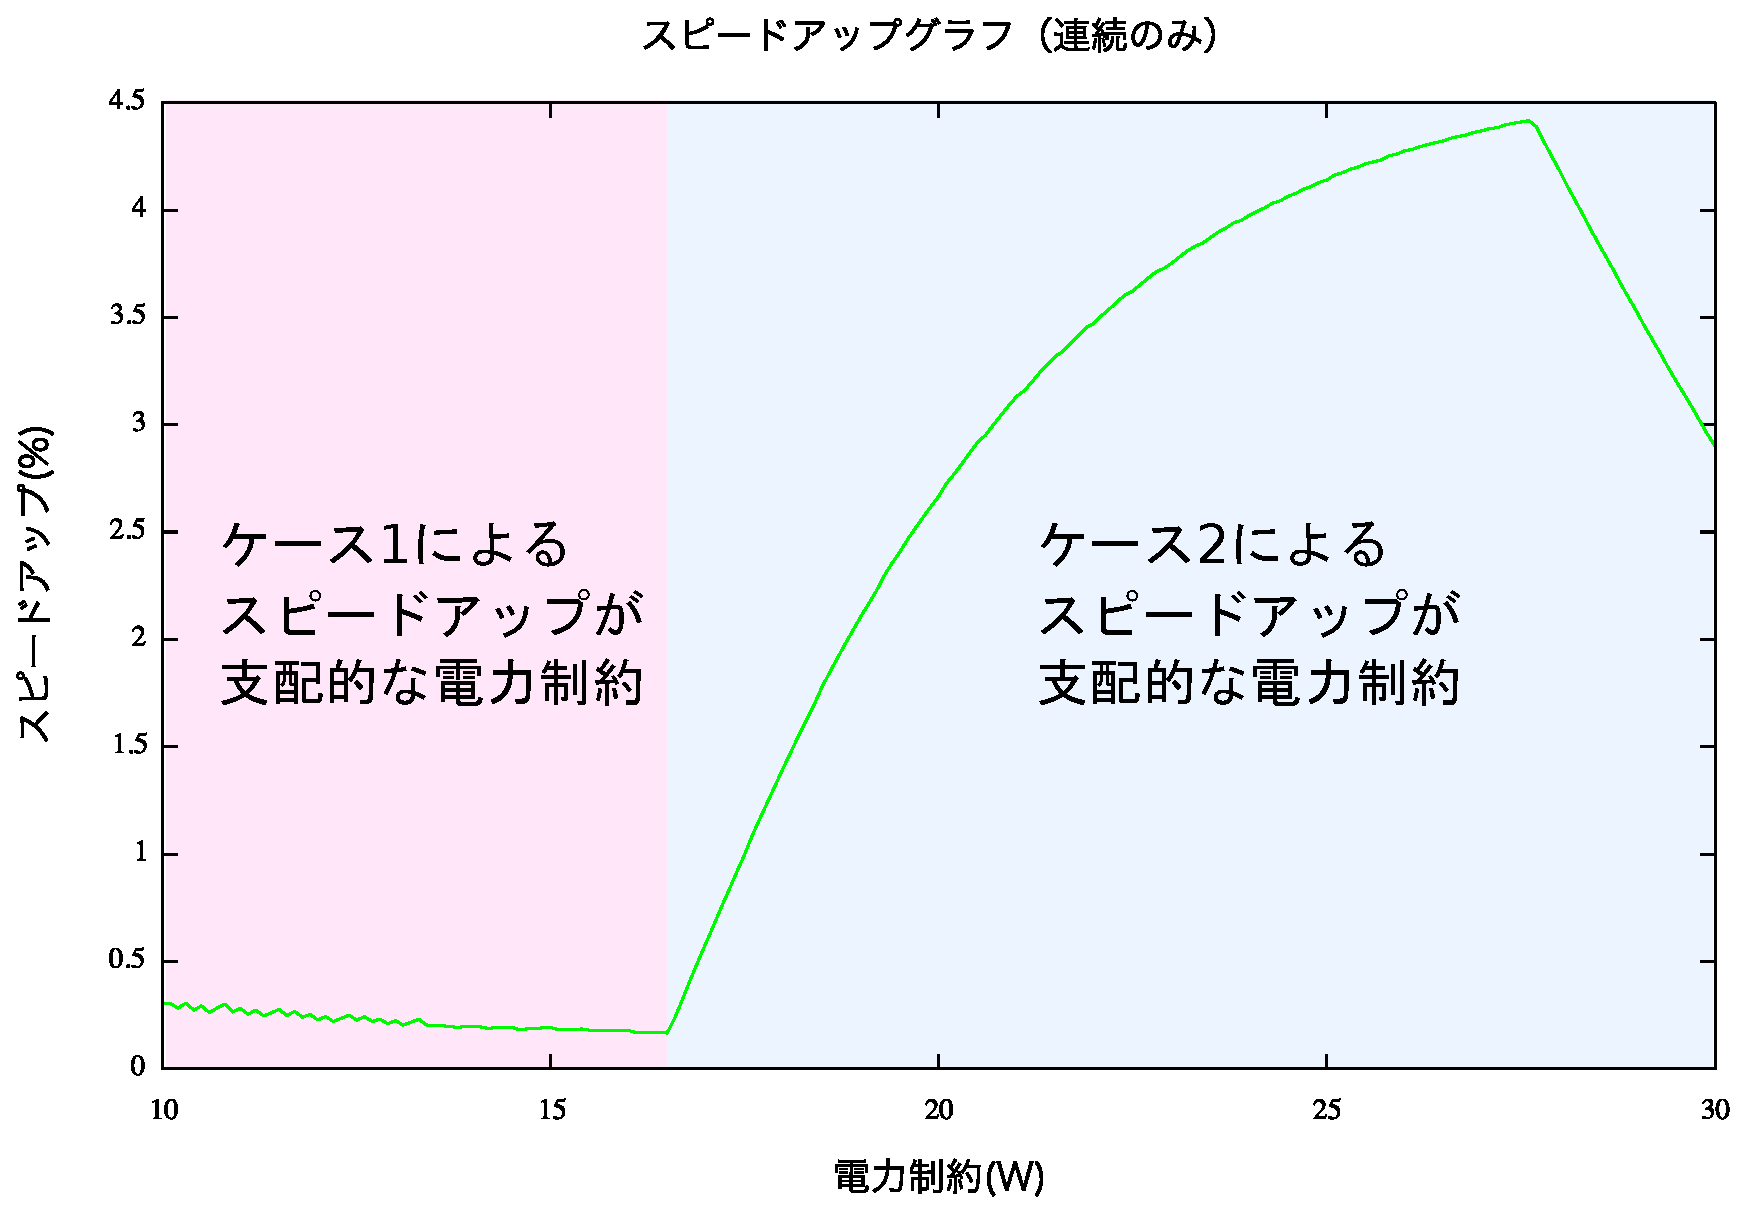
\includegraphics[width=123mm]{canneal_speedup_continuous_modified.eps}
 \end{center}
 \caption{Canneal 電力融通を行わない場合と比べた性能向上(連続の場合のみ)}
 \label{fig:canneal_speedup_continuous}
\end{figure}

\begin{figure}[t]
 \begin{center}
  \includegraphics[width=123mm]{frequency_transition_canneal.eps}
 \end{center}
 \caption{Canneal 周波数の推移の様子(連続の場合)}
 \label{fig:frequency_transition_canneal}
\end{figure}

\begin{figure}[t]
 \begin{center}
  \includegraphics[width=123mm]{mummergpu_speedup_discrete_modified.eps}
 \end{center}
 \caption{mummergpu 電力融通を行わない場合と比べた性能向上(離散の場合のみ)}
 \label{fig:mummergpu_speedup_discrete}
\end{figure}

\begin{figure}[t]
 \begin{center}
  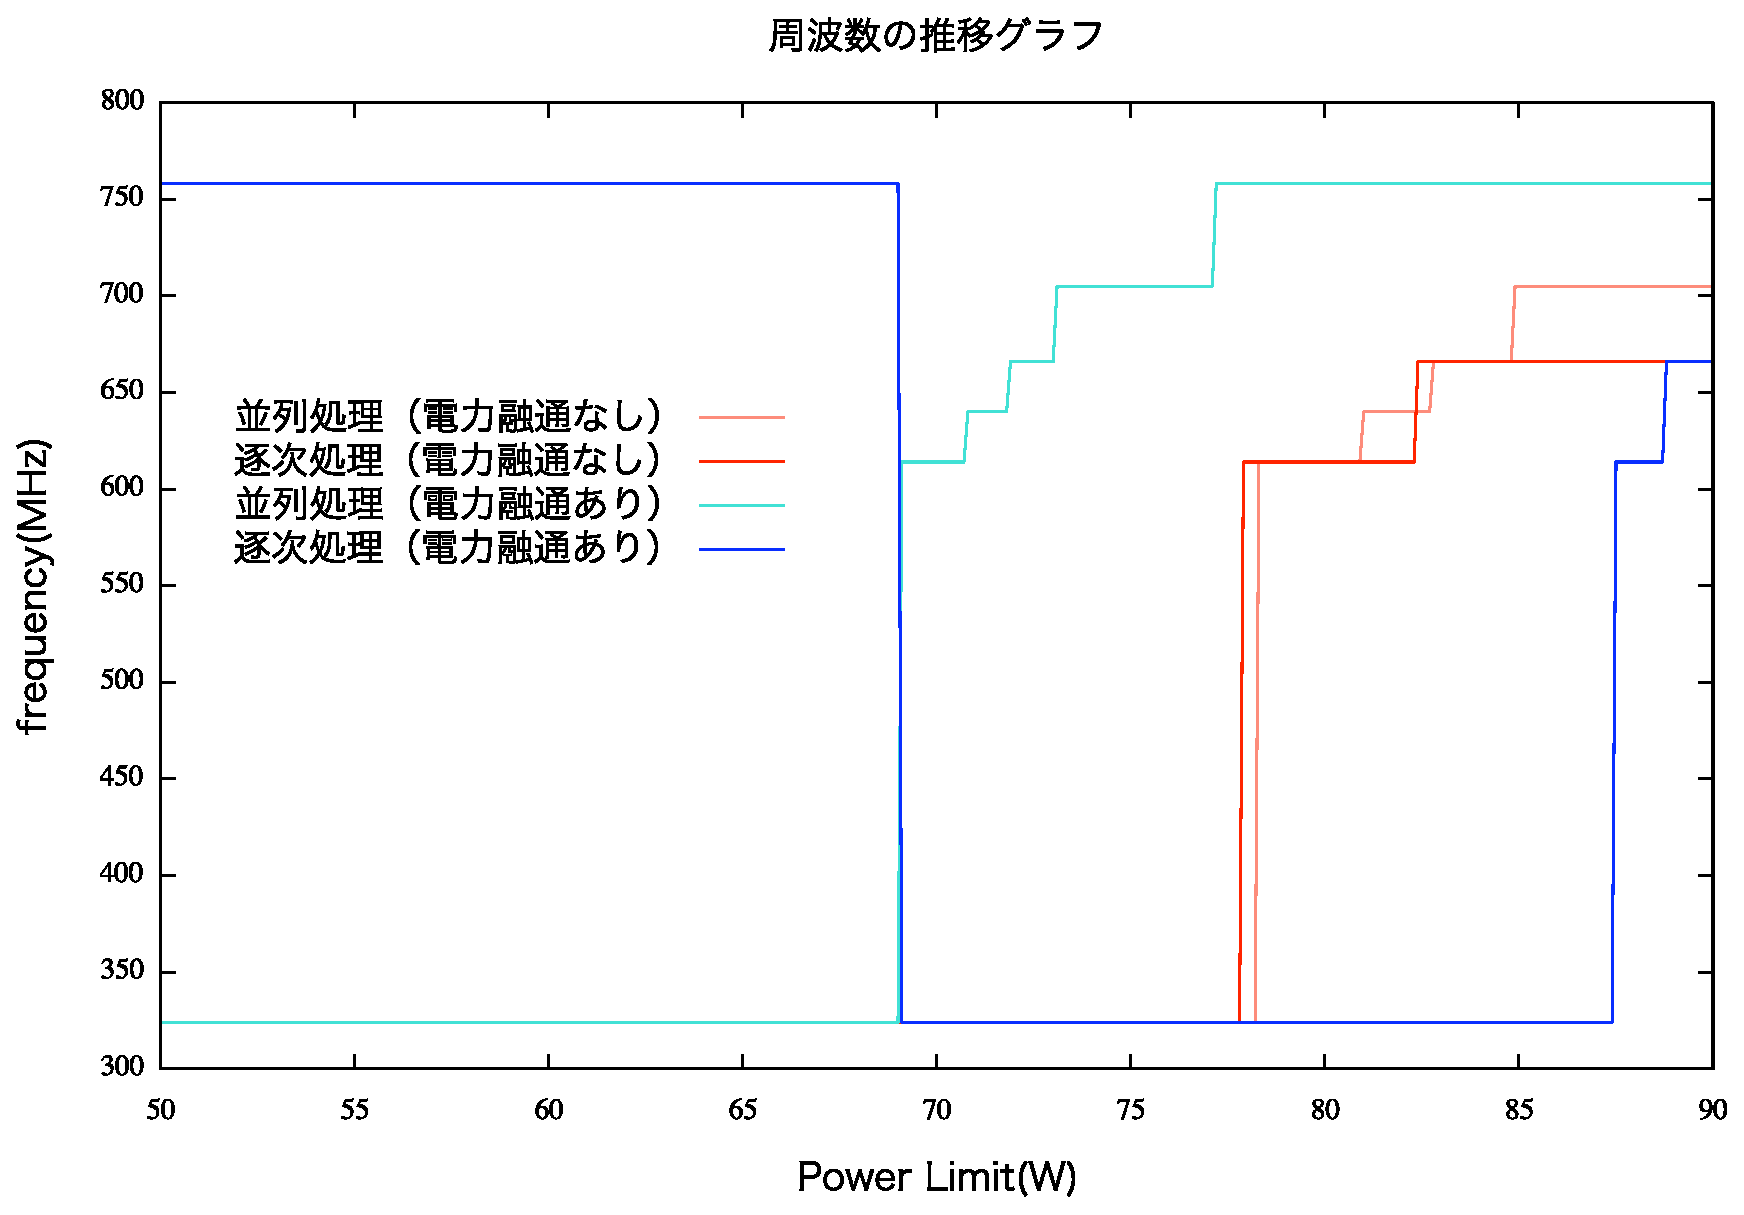
\includegraphics[width=123mm]{frequency_transition_mummergpu.eps}
 \end{center}
 \caption{mummergpu 周波数の推移の様子(離散の場合)}
 \label{fig:frequency_transition_mummergpu}
\end{figure}


\section{考察}
\label{sec:discussion}

4つのアプリケーションの中で、Stream Clusterのみは性能向上がとても小さかった。これは、逐次処理部分の実行時間が並列処理部分の実行時間と比べて非常に短かったため、蓄電池が充放電する時間がほとんどなく、電力融通を上手く行うことができなかったためであると考えられる。

\subsection{周波数が連続的な値を取れる理想的なプロセッサの場合の考察}
\label{subsec:continuous}


連続的に周波数が変更できる場合にどのような周波数が最適解となっているかについて考察する。ここでは比較的説明のしやすい、Cannealの連続補間した場合の結果について説明する。

図\ref{fig:canneal_speedup_continuous}、\ref{fig:frequency_transition_canneal}はそれぞれ、周波数が連続的に変えられる場合のCannealの電力−実行時間曲線と性能向上の様子である。図\ref{fig:canneal_speedup_continuous}を見ると、電力制約が17Wの部分から性能向上率が増加し始め、28W付近でピークに達しその後は減少していくのが分かる。

まず、電力制約が17Wより小さいときの最適周波数について考える。図\ref{fig:canneal_speedup_continuous}に示したようにこの電力制約においては、ケース1による効果が支配的である。これは図\ref{fig:frequency_transition_canneal}を見ると分かるように、この電力制約においては、どちらも周波数の上限・下限には達しておらず、ケース2の効果はないためである。また、逐次処理の周波数を下げて並列処理の周波数を上げていることから、逐次処理部分は電力を上げても実行時間があまり短縮されないフェーズであり、逆に並列処理部分は電力を上げることで実行時間が大きく短縮されるフェーズであったということが分かる。

ここで、ケース1におけるそれぞれのフェーズの周波数はどのような法則によって決められているのかを考察する。注意すべきは、蓄電池によって融通しているものは電力ではなくエネルギであるという点である。フェーズAで10Wで充電できたからといって、フェーズBで10Wで放電できるとは限らない。これはそれぞれのフェーズの実行時間が異なるため、充放電されるエネルギに差が生じるためである。しかし、\ref{sec:formularization}節で述べたような理想的な蓄電池の場合にはフェーズAで10J充電できた場合はフェーズBで必ず10J放電することができる。つまり、それぞれのフェーズにかけるエネルギを微小変化させたときの、実行時間の短縮の大きさを見てやればよいことになる。これは、実行時間を実行エネルギで微分したものを正負逆転させたものに他ならない。これをエネルギ実行時間短縮率と呼ぶこととする。エネルギ実行時間短縮率は式\ref{asm:model}を用いて以下のように求められる。

\begin{eqnarray}
E &=& p \cdot T(p)\\
-\frac{dT}{dE} &=& -\frac{dT}{dp} \bigg/ \frac{dE}{dp}\\
&=& -\frac{1}{a_2 - \cfrac{a_0}{a_1}( p-a_2)^2} \label{asm:differential}
\end{eqnarray}

実際に17W以下の部分については、式\ref{asm:differential}の値がほぼ一致していた。つまりこの部分については、それぞれのフェーズのエネルギ実行時間短縮率の一致する部分が最適解となっている。また、この部分における性能向上率は0.5\%未満とかなり小さい。

次に17-28Wの部分について考える。図\ref{fig:canneal_speedup_continuous}に示したようにこの電力制約においてはケース2の効果が支配的である。図\ref{fig:frequency_transition_canneal}を見ると、17Wのときに電力融通をしない場合の逐次処理部分での動作周波数が頭打ちになり、実行時間が短くならなくなることが分かる。一方で電力融通を行う場合には頭打ちになるのがもう少し遅く、頭打ちになってもその部分で余った電力を並列部分へ融通して周波数を上げることができるので、実行時間は短くなり続ける。そのため実行時間の差は開き続け、性能向上率が大きくなり続ける。

この電力制約における最適周波数での式\ref{asm:differential}の値を見ると、逐次処理の値の方が小さい。これは逐次処理の方がエネルギ実行時間短縮率が大きいことを意味しているため、もし逐次処理の周波数をさらに上げることができれば、並列処理部分での動作周波数を下げ、代わりに逐次処理部分では動作周波数を上げていたと予想される。

最後に28W以上の部分について考える。この部分についての説明は容易である。図\ref{fig:frequency_transition_canneal}から、28Wのときに電力融通を行っている場合には逐次処理・並列処理のどちらのフェーズも動作周波数が頭打ちになる。従って、電力融通をしている場合にはこれ以上実行時間を短縮する余地がない。一方で電力融通していない場合には、並列処理部分の動作周波数をまだ上げることができるため、実行時間が短縮されていく。結果として性能向上率は減少していく。

以上それぞれのフェーズにおける考察より、プロセッサが連続的な周波数で動作できる場合にはエネルギ実行時間短縮率が高いフェーズから低いフェーズへできる限り電力を融通できるような充放電計画が最適となることが分かる。また、17W以下の部分の性能向上率を見れば分かるように、電力−実行時間曲線の特性の違いによって生じるエネルギ実行時間短縮率の違いを利用した電力融通だけでは効果は小さい。一方で17W以上の部分のように、一方のフェーズにおけるプロセッサの性能が頭打ちになることによる余剰電力などがあれば大きな性能向上が見込める。

\subsection{周波数が離散的な値のみしかとれない現実のプロセッサの場合の考察}
\label{subsec:discrete}

離散の場合には電力制約によってはところどころ針が立ったように大きく性能向上している部分がある。これはケース3の効果に分類されるもので、もう少し電力制約が大きくなればもう一つ上の周波数に上げることができる、という状況で起こるものである。逐次処理でわずかに蓄えたエネルギを並列処理部分に融通することで、周波数を一段階上げることができたのである。周波数が連続的に変えられる場合には、周波数を数段階上げる程度では大した時間短縮にはならないため、このようなことは起こらない。

全てのアプリケーションを通して、離散的な周波数しか取れない場合の方が連続的に周波数を変化させられる場合に比べて効果は大きかった。これは\ref{sec:curb}節で述べたように、周波数が離散的であるために生じる余剰電力を蓄電池を用いて融通することによる性能向上効果のためであると考えられる。

全体的に、離散的な周波数しか取れない場合には電力制約ごとに性能向上率の値が大きく異なる。これまでに述べたように離散的であると余剰電力は多く生じるのだが、周波数を一段階上げるために必要なエネルギ融通量も大きくなる。また、周波数を一段階上げたときに短縮される実行時間も大きい。そのため、電力融通により上手く周波数を上げられるような電力制約の場合は大きく性能向上する一方で、逆に周波数を上手く上げられないような電力制約ではほとんど性能向上させることができないのである。

また、電力制約ごとにケース1、2、3のどの効果がどれほど性能向上率に影響しているかを定量的に評価することはできなかった。それぞれの効果がお互いに影響し合っており、分離することが実質的に困難なためである。

以上のことをまとめると、周波数が離散的である場合に効果があるのは、電力制約がサポートされているいずれかの動作周波数よりわずかに小さいような場合である。この場合には他のフェーズの余剰電力を蓄電池で融通することで周波数を上げることができる可能性が高いため、実行時間が大きく短縮される。逆に効果が薄いのは電力制約がいずれかの動作周波数と同じか、わずかに大きい場合である。この場合には次の周波数まで大きなギャップがある上、余剰電力もあまり生じないため電力融通を上手く行うことができない。


\subsection{全体の考察}
\label{sebsec:whole}

今回の実験の結果、離散的な周波数しか取れないプロセッサ上において、同程度の実行時間のフェーズを複数有するアプリケーションに本手法を適用することで、CPU上で実行されるアプリケーションでは平均4.5\%、GPU上で実行されるアプリケーションでは平均17.1\%の実行時間の短縮がなされることが分かった。\ref{sec:curb}節で述べたケース1、2、3のそれぞれの効果がどれくらい実行時間の短縮に寄与したかを定量的に評価するには至らなかった。ただし、図\ref{fig:canneal_speedup_continuous}、\ref{fig:mummergpu_speedup_discrete}におけるそれぞれの効果を見る限りでは、ケース2、3の実行時間短縮効果はケース1に比べて大きいようであった。

今回の実験では電力融通問題を解くために全探索で最適解を求めた。$n$個のフェーズがあるアプリケーションを、$m$個の動作周波数をサポートしているプロセッサ上で走らせた場合の最適解を全探索で求めると、その計算量は${\rm O}(m^n)$となる。これは非常に大きな計算量であるため、新たなアルゴリズムの構築が求められる。そのため、今後は\ref{subsec:continuous}節で述べたようなエネルギ実行時間短縮率を指標とした計算量の小さなアルゴリズムの考案が課題となるであろう。また今回は理想的な蓄電池を想定したが、蓄電池の電池容量や充放電速度などの物理的制約を考慮に入れたアルゴリズムの構築も課題である。











\chapter{結果及び考察}
\label{chap:result}


\section{電力制約下における性能向上率}
\label{sec:speedup}

\section{フェーズ分割アルゴリズムの評価}
\label{sec:evaluate_algorithm}

\section{充放電計画決定アルゴリズムの評価}
\label{sec:evaluate_plan}

\section{全体の考察}
\label{sec:discussion}
\chapter{結論}
\label{chap:conclusion}





\backmatter% ここから後付
\chapter{謝辞}%%%%%%%%%%%%%%% 謝辞 %%%%%%%

\begin{thebibliography}{}%%%% 参考文献 %%%
 \bibitem{}
\end{thebibliography}
%\bibliographystyle{}%           BibTeX を使う場合
%\bibliography{.bib ファイル名}% BibTeX を使う場合

\appendix% ここから付録 %%%%% 付録 %%%%%%%
\chapter{}
\end{document}
